\section[ML overview]{Machine learning overview}

\subsection{}

\begin{frame}
    \frametitle{What is machine learning?}

    \begin{block}{My definition}
        The study of computational algorithms
        \begin{itemize}
            \item that \alert{predict} outputs from inputs;
            \item whose behavior is determined by \alert{model parameters};
            \item that \alert{learn} how to make predictions by fitting (``training'') the model parameters to data;
            \item that \alert{iteratively} improve their model parameters via continual training.
        \end{itemize}
    \end{block}

    \begin{columns}
        \begin{column}{2.5in}
            Simplest example: linear regression
            \begin{itemize}
                \item Sort of: not iterative
                \item Predicts $y$ from $x$ via $y = ax + b$
                \item Two parameters: $a$, $b$
                \item Fitted to data
            \end{itemize}
        \end{column}
        \begin{column}{1.75in}
            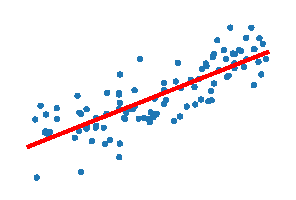
\includegraphics{linear_regression}
        \end{column}
    \end{columns}
\end{frame}

\begin{frame}
    \frametitle{A (much) more complicated example}
    \begin{columns}
        \begin{column}{0.37\textwidth}
            \begin{block}{Image classification}
                A canonical problem: given an image, predict the correct label
            \end{block}
        \end{column}
        \begin{column}{0.63\textwidth}
            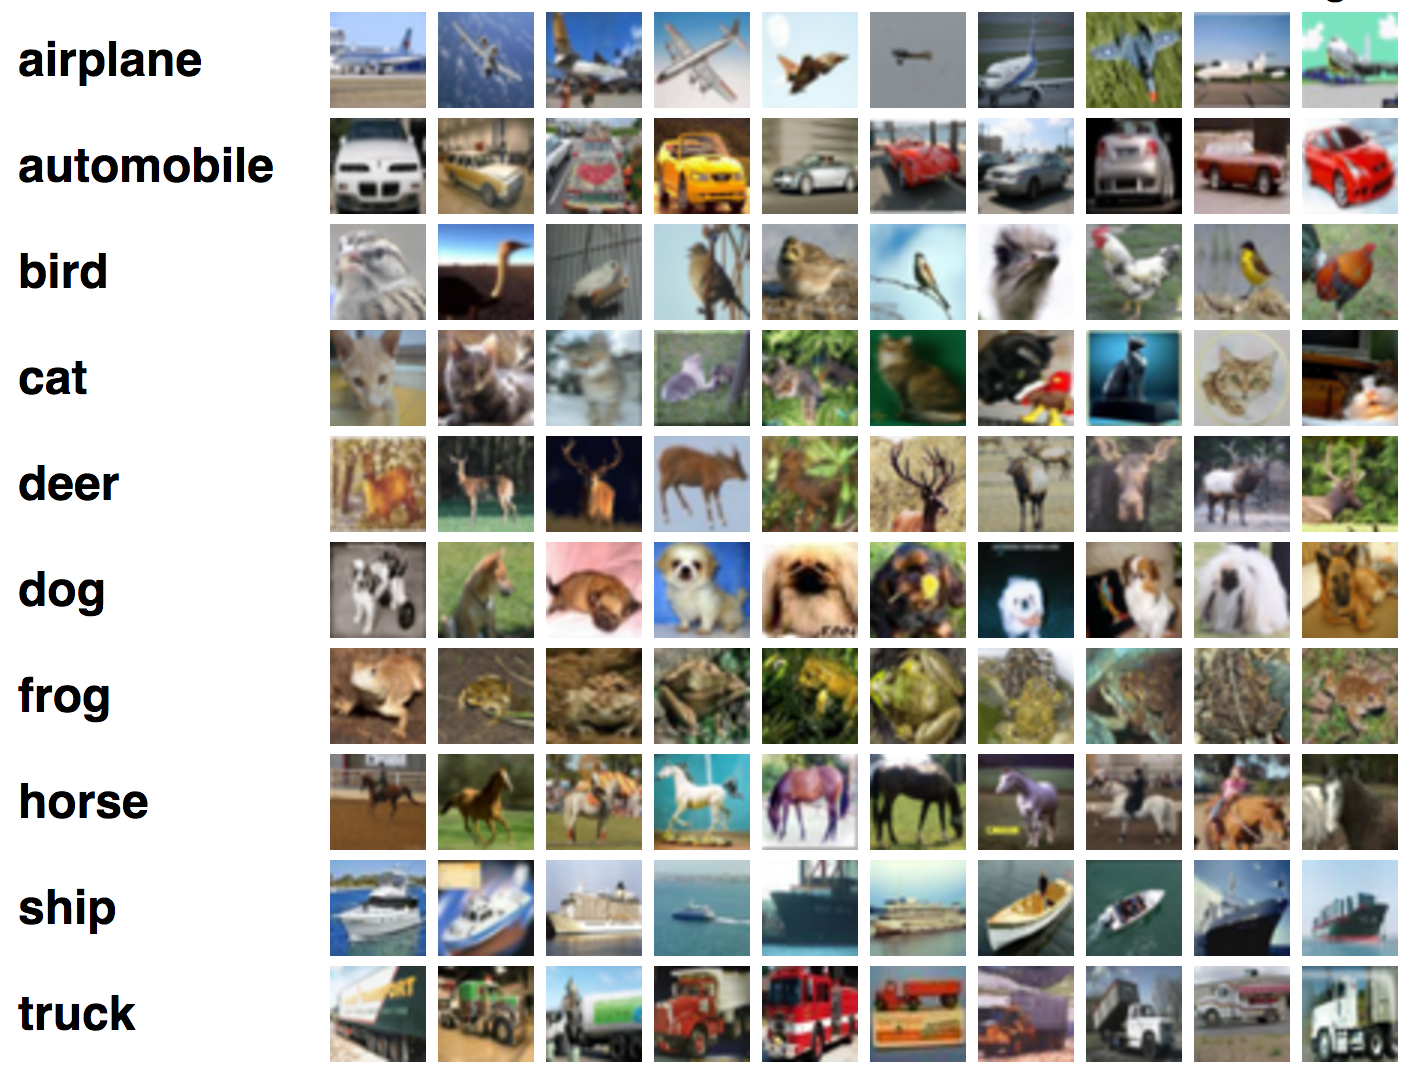
\includegraphics[width=\textwidth]{cifar10}
        \end{column}
    \end{columns}

    \begin{itemize}
        \item Roughly: if a human can do it, a computer should be able to too
        \item More rigorously: $\exists$ a mapping from image pixels to labels
        \begin{itemize}
            \item Mapping too difficult for humans to understand
            \item Let an algorithm model it
        \end{itemize}
    \end{itemize}
\end{frame}

\begin{frame}
    \frametitle{An image classification solution}

    \begin{columns}
        \begin{column}{0.7\textwidth}
            ResNet-152: a 152-layer convolutional neural network with 11.3 billion multiply/adds! \citep{He15}
            \begin{itemize}
                \item Trained on ImageNet data: 14,197,122 images
                \item Iterative training
                \begin{itemize}
                    \item 600,000 training iterations
                    \item At each iteration, model parameters updated based on \emph{mini-batch} of 256 images
                \end{itemize}
                \item Won multiple image classification competitions
            \end{itemize}
        \end{column}
        \begin{column}{0.3\textwidth}
            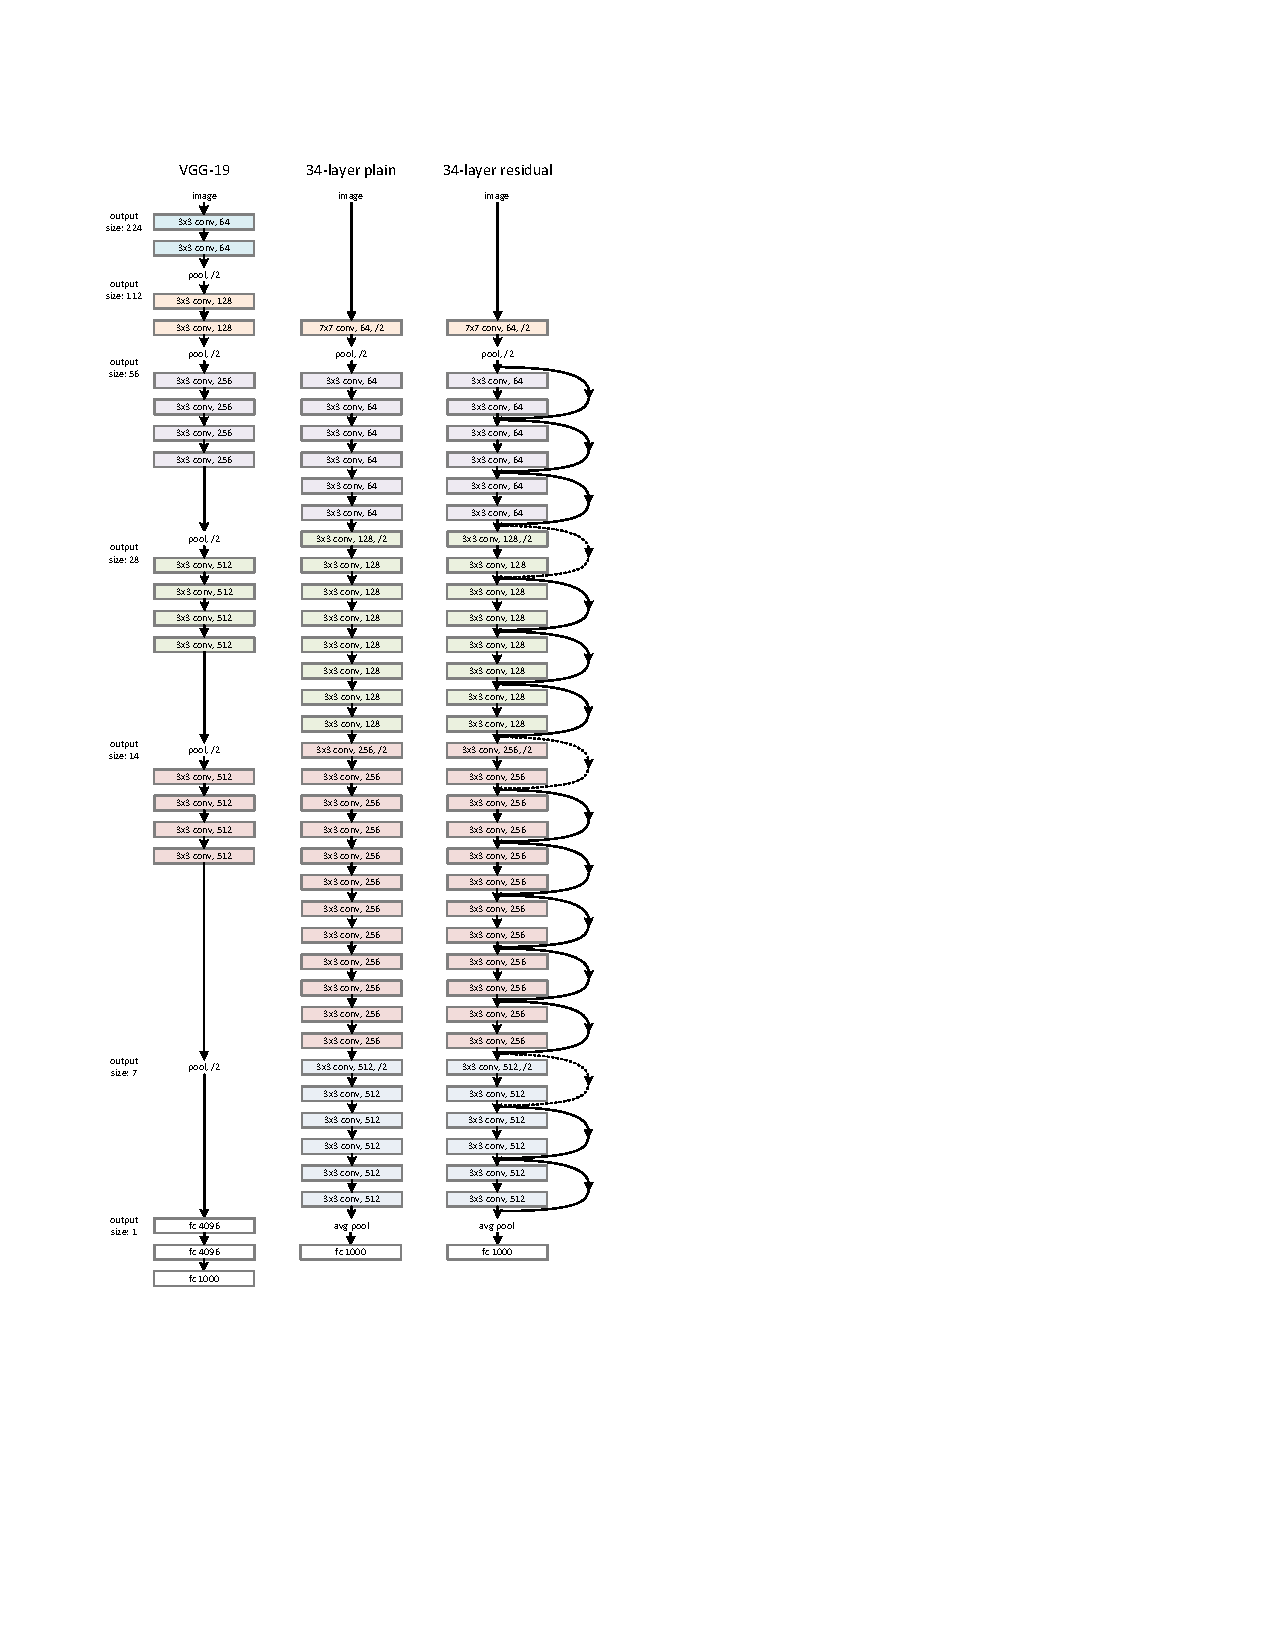
\includegraphics[width=\textwidth]{resnet}
        \end{column}
    \end{columns}
\end{frame}

\begin{frame}
    \frametitle{Supervised vs.\ unsupervised learning}
    
\end{frame}

\begin{frame}
    \frametitle{Regression vs.\ classification}
    
\end{frame}

% Universal approximation
% Quick thing on decision trees

%%% Local Variables:
%%% mode: latex
%%% TeX-master: "../nn"
%%% End:
